\documentclass[../tex_main/NEMO_manual]{subfiles}
\begin{document}
% ================================================================
% Chapter ——— Ocean Dynamics (DYN)
% ================================================================
\chapter{Ocean Dynamics (DYN)}
\label{chap:DYN}
\minitoc

%\vspace{2.cm}
$\ $\newline      %force an empty line

Using the representation described in \autoref{chap:DOM},
several semi-discrete space forms of the dynamical equations are available depending on
the vertical coordinate used and on the conservation properties of the vorticity term.
In all the equations presented here, the masking has been omitted for simplicity.
One must be aware that all the quantities are masked fields and
that each time an average or difference operator is used, the resulting field is multiplied by a mask.

The prognostic ocean dynamics equation can be summarized as follows:
\begin{equation*}
\text{NXT} = \dbinom	{\text{VOR} + \text{KEG} + \text {ZAD} }
						{\text{COR} + \text{ADV}                       }
			+ \text{HPG} + \text{SPG} + \text{LDF} + \text{ZDF}
\end{equation*}
NXT stands for next, referring to the time-stepping.
The first group of terms on the rhs of this equation corresponds to the Coriolis and advection terms that
are decomposed into either a vorticity part (VOR), a kinetic energy part (KEG) and
a vertical advection part (ZAD) in the vector invariant formulation,
or a Coriolis and advection part (COR+ADV) in the flux formulation.
The terms following these are the pressure gradient contributions
(HPG, Hydrostatic Pressure Gradient, and SPG, Surface Pressure Gradient);
and contributions from lateral diffusion (LDF) and vertical diffusion (ZDF),
which are added to the rhs in the \mdl{dynldf} and \mdl{dynzdf} modules.
The vertical diffusion term includes the surface and bottom stresses.
The external forcings and parameterisations require complex inputs
(surface wind stress calculation using bulk formulae, estimation of mixing coefficients)
that are carried out in modules SBC, LDF and ZDF and are described in
\autoref{chap:SBC}, \autoref{chap:LDF} and \autoref{chap:ZDF}, respectively. 

In the present chapter we also describe the diagnostic equations used to compute the horizontal divergence,
curl of the velocities (\emph{divcur} module) and the vertical velocity (\emph{wzvmod} module).

The different options available to the user are managed by namelist variables. 
For term \textit{ttt} in the momentum equations, the logical namelist variables are \textit{ln\_dynttt\_xxx}, 
where \textit{xxx} is a 3 or 4 letter acronym corresponding to each optional scheme.
If a CPP key is used for this term its name is \key{ttt}.
The corresponding code can be found in the \textit{dynttt\_xxx} module in the DYN directory,
and it is usually computed in the \textit{dyn\_ttt\_xxx} subroutine.

The user has the option of extracting and outputting each tendency term from the 3D momentum equations
(\key{trddyn} defined), as described in \autoref{chap:MISC}.
Furthermore, the tendency terms associated with the 2D barotropic vorticity balance (when \key{trdvor} is defined)
can be derived from the 3D terms.
%%%
\gmcomment{STEVEN: not quite sure I've got the sense of the last sentence. does 
MISC correspond to "extracting tendency terms" or "vorticity balance"?}

$\ $\newline    % force a new ligne

% ================================================================
% Sea Surface Height evolution & Diagnostics variables
% ================================================================
\section{Sea surface height and diagnostic variables ($\eta$, $\zeta$, $\chi$, $w$)}
\label{sec:DYN_divcur_wzv}

%--------------------------------------------------------------------------------------------------------------
%           Horizontal divergence and relative vorticity
%--------------------------------------------------------------------------------------------------------------
\subsection{Horizontal divergence and relative vorticity (\protect\mdl{divcur})}
\label{subsec:DYN_divcur}

The vorticity is defined at an $f$-point ($i.e.$ corner point) as follows:
\begin{equation} \label{eq:divcur_cur}
\zeta =\frac{1}{e_{1f}\,e_{2f} }\left( {\;\delta _{i+1/2} \left[ {e_{2v}\;v} \right]
						        -\delta _{j+1/2} \left[ {e_{1u}\;u} \right]\;} \right)
\end{equation} 

The horizontal divergence is defined at a $T$-point.
It is given by:
\begin{equation} \label{eq:divcur_div}
\chi =\frac{1}{e_{1t}\,e_{2t}\,e_{3t} }
		\left( {\delta _i \left[ {e_{2u}\,e_{3u}\,u} \right]
		       +\delta _j \left[ {e_{1v}\,e_{3v}\,v} \right]} \right)
\end{equation} 

Note that although the vorticity has the same discrete expression in $z$- and $s$-coordinates,
its physical meaning is not identical.
$\zeta$ is a pseudo vorticity along $s$-surfaces
(only pseudo because $(u,v)$ are still defined along geopotential surfaces,
but are not necessarily defined at the same depth).

The vorticity and divergence at the \textit{before} step are used in the computation of
the horizontal diffusion of momentum.
Note that because they have been calculated prior to the Asselin filtering of the \textit{before} velocities,
the \textit{before} vorticity and divergence arrays must be included in the restart file to
ensure perfect restartability.
The vorticity and divergence at the \textit{now} time step are used for the computation of
the nonlinear advection and of the vertical velocity respectively. 

%--------------------------------------------------------------------------------------------------------------
%           Sea Surface Height evolution
%--------------------------------------------------------------------------------------------------------------
\subsection{Horizontal divergence and relative vorticity (\protect\mdl{sshwzv})}
\label{subsec:DYN_sshwzv}

The sea surface height is given by:
\begin{equation} \label{eq:dynspg_ssh}
\begin{aligned}
\frac{\partial \eta }{\partial t}
&\equiv    \frac{1}{e_{1t} e_{2t} }\sum\limits_k { \left\{  \delta _i \left[ {e_{2u}\,e_{3u}\;u} \right]
                                                                                  +\delta _j \left[ {e_{1v}\,e_{3v}\;v} \right]  \right\} } 
           -    \frac{\textit{emp}}{\rho _w }   \\
&\equiv    \sum\limits_k {\chi \ e_{3t}}  -  \frac{\textit{emp}}{\rho _w }
\end{aligned}
\end{equation}
where \textit{emp} is the surface freshwater budget (evaporation minus precipitation), 
expressed in Kg/m$^2$/s (which is equal to mm/s),
and $\rho _w$=1,035~Kg/m$^3$ is the reference density of sea water (Boussinesq approximation).
If river runoff is expressed as a surface freshwater flux (see \autoref{chap:SBC}) then
\textit{emp} can be written as the evaporation minus precipitation, minus the river runoff. 
The sea-surface height is evaluated using exactly the same time stepping scheme as
the tracer equation \autoref{eq:tra_nxt}:
a leapfrog scheme in combination with an Asselin time filter,
$i.e.$ the velocity appearing in \autoref{eq:dynspg_ssh} is centred in time (\textit{now} velocity).
This is of paramount importance.
Replacing $T$ by the number $1$ in the tracer equation and summing over the water column must lead to
the sea surface height equation otherwise tracer content will not be conserved
\citep{Griffies_al_MWR01, Leclair_Madec_OM09}.

The vertical velocity is computed by an upward integration of the horizontal divergence starting at the bottom,
taking into account the change of the thickness of the levels:
\begin{equation} \label{eq:wzv}
\left\{   \begin{aligned}
&\left. w \right|_{k_b-1/2} \quad= 0    \qquad \text{where } k_b \text{ is the level just above the sea floor }  	\\
&\left. w \right|_{k+1/2}     = \left. w \right|_{k-1/2}  +  \left. e_{3t} \right|_{k}\;  \left. \chi \right|_k  
                                         - \frac{1} {2 \rdt} \left(  \left. e_{3t}^{t+1}\right|_{k} - \left. e_{3t}^{t-1}\right|_{k}\right)
\end{aligned}   \right.
\end{equation}

In the case of a non-linear free surface (\key{vvl}), the top vertical velocity is $-\textit{emp}/\rho_w$, 
as changes in the divergence of the barotropic transport are absorbed into the change of the level thicknesses,
re-orientated downward.
\gmcomment{not sure of this...  to be modified with the change in emp setting}
In the case of a linear free surface, the time derivative in \autoref{eq:wzv} disappears.
The upper boundary condition applies at a fixed level $z=0$.
The top vertical velocity is thus equal to the divergence of the barotropic transport
($i.e.$ the first term in the right-hand-side of \autoref{eq:dynspg_ssh}).

Note also that whereas the vertical velocity has the same discrete expression in $z$- and $s$-coordinates,
its physical meaning is not the same:
in the second case, $w$ is the velocity normal to the $s$-surfaces.
Note also that the $k$-axis is re-orientated downwards in the \textsc{fortran} code compared to
the indexing used in the semi-discrete equations such as \autoref{eq:wzv}
(see \autoref{subsec:DOM_Num_Index_vertical}). 


% ================================================================
% Coriolis and Advection terms: vector invariant form
% ================================================================
\section{Coriolis and advection: vector invariant form}
\label{sec:DYN_adv_cor_vect}
%-----------------------------------------nam_dynadv----------------------------------------------------

\nlst{namdyn_adv} 
%-------------------------------------------------------------------------------------------------------------

The vector invariant form of the momentum equations is the one most often used in
applications of the \NEMO ocean model.
The flux form option (see next section) has been present since version $2$.
Options are defined through the \ngn{namdyn\_adv} namelist variables Coriolis and
momentum advection terms are evaluated using a leapfrog scheme,
$i.e.$ the velocity appearing in these expressions is centred in time (\textit{now} velocity). 
At the lateral boundaries either free slip, no slip or partial slip boundary conditions are applied following
\autoref{chap:LBC}.

% -------------------------------------------------------------------------------------------------------------
%        Vorticity term 
% -------------------------------------------------------------------------------------------------------------
\subsection{Vorticity term (\protect\mdl{dynvor})}
\label{subsec:DYN_vor}
%------------------------------------------nam_dynvor----------------------------------------------------

\nlst{namdyn_vor} 
%-------------------------------------------------------------------------------------------------------------

Options are defined through the \ngn{namdyn\_vor} namelist variables.
Four discretisations of the vorticity term (\np{ln\_dynvor\_xxx}\forcode{ = .true.}) are available:
conserving potential enstrophy of horizontally non-divergent flow (ENS scheme);
conserving horizontal kinetic energy (ENE scheme);
conserving potential enstrophy for the relative vorticity term and
horizontal kinetic energy for the planetary vorticity term (MIX scheme);
or conserving both the potential enstrophy of horizontally non-divergent flow and horizontal kinetic energy
(EEN scheme) (see \autoref{subsec:C_vorEEN}).
In the case of ENS, ENE or MIX schemes the land sea mask may be slightly modified to ensure the consistency of
vorticity term with analytical equations (\np{ln\_dynvor\_con}\forcode{ = .true.}).
The vorticity terms are all computed in dedicated routines that can be found in the \mdl{dynvor} module.

%-------------------------------------------------------------
%                 enstrophy conserving scheme
%-------------------------------------------------------------
\subsubsection{Enstrophy conserving scheme (\protect\np{ln\_dynvor\_ens}\forcode{ = .true.})}
\label{subsec:DYN_vor_ens}

In the enstrophy conserving case (ENS scheme),
the discrete formulation of the vorticity term provides a global conservation of the enstrophy
($ [ (\zeta +f ) / e_{3f} ]^2 $ in $s$-coordinates) for a horizontally non-divergent flow ($i.e.$ $\chi$=$0$),
but does not conserve the total kinetic energy.
It is given by:
\begin{equation} \label{eq:dynvor_ens}
\left\{ 
\begin{aligned}
{+\frac{1}{e_{1u} } } & {\overline {\left( { \frac{\zeta +f}{e_{3f} }} \right)} }^{\,i} 
                                & {\overline{\overline {\left( {e_{1v}\,e_{3v}\;v} \right)}} }^{\,i, j+1/2}    \\
{- \frac{1}{e_{2v} } } & {\overline {\left( {\frac{\zeta +f}{e_{3f} }} \right)} }^{\,j}  
                                & {\overline{\overline {\left( {e_{2u}\,e_{3u}\;u} \right)}} }^{\,i+1/2, j}  
\end{aligned} 
 \right.
\end{equation} 

%-------------------------------------------------------------
%                 energy conserving scheme
%-------------------------------------------------------------
\subsubsection{Energy conserving scheme (\protect\np{ln\_dynvor\_ene}\forcode{ = .true.})}
\label{subsec:DYN_vor_ene}

The kinetic energy conserving scheme (ENE scheme) conserves the global kinetic energy but not the global enstrophy.
It is given by:
\begin{equation} \label{eq:dynvor_ene}
\left\{   \begin{aligned}
{+\frac{1}{e_{1u}}\; {\overline {\left( {\frac{\zeta +f}{e_{3f} }} \right)
                            \;  \overline {\left( {e_{1v}\,e_{3v}\;v} \right)} ^{\,i+1/2}} }^{\,j} }    \\
{- \frac{1}{e_{2v}}\; {\overline {\left( {\frac{\zeta +f}{e_{3f} }} \right)
                            \;  \overline {\left( {e_{2u}\,e_{3u}\;u} \right)} ^{\,j+1/2}} }^{\,i} }
\end{aligned}    \right.
\end{equation} 

%-------------------------------------------------------------
%                 mix energy/enstrophy conserving scheme
%-------------------------------------------------------------
\subsubsection{Mixed energy/enstrophy conserving scheme (\protect\np{ln\_dynvor\_mix}\forcode{ = .true.}) }
\label{subsec:DYN_vor_mix}

For the mixed energy/enstrophy conserving scheme (MIX scheme), a mixture of the two previous schemes is used.
It consists of the ENS scheme (\autoref{eq:dynvor_ens}) for the relative vorticity term,
and of the ENE scheme (\autoref{eq:dynvor_ene}) applied to the planetary vorticity term.
\begin{equation} \label{eq:dynvor_mix}
\left\{ {     \begin{aligned}
 {+\frac{1}{e_{1u} }\; {\overline {\left( {\frac{\zeta }{e_{3f} }} \right)} }^{\,i} 
 \; {\overline{\overline {\left( {e_{1v}\,e_{3v}\;v} \right)}} }^{\,i,j+1/2} -\frac{1}{e_{1u} }
 \; {\overline {\left( {\frac{f}{e_{3f} }} \right) 
 \;\overline {\left( {e_{1v}\,e_{3v}\;v} \right)} ^{\,i+1/2}} }^{\,j} } \\
{-\frac{1}{e_{2v} }\; {\overline {\left( {\frac{\zeta }{e_{3f} }} \right)} }^j
 \; {\overline{\overline {\left( {e_{2u}\,e_{3u}\;u} \right)}} }^{\,i+1/2,j} +\frac{1}{e_{2v} }
 \; {\overline {\left( {\frac{f}{e_{3f} }} \right)
 \;\overline {\left( {e_{2u}\,e_{3u}\;u} \right)} ^{\,j+1/2}} }^{\,i} } \hfill
\end{aligned}     } \right.
\end{equation} 

%-------------------------------------------------------------
%                 energy and enstrophy conserving scheme
%-------------------------------------------------------------
\subsubsection{Energy and enstrophy conserving scheme (\protect\np{ln\_dynvor\_een}\forcode{ = .true.}) }
\label{subsec:DYN_vor_een}

In both the ENS and ENE schemes,
it is apparent that the combination of $i$ and $j$ averages of the velocity allows for
the presence of grid point oscillation structures that will be invisible to the operator.
These structures are \textit{computational modes} that will be at least partly damped by
the momentum diffusion operator ($i.e.$ the subgrid-scale advection), but not by the resolved advection term.
The ENS and ENE schemes therefore do not contribute to dump any grid point noise in the horizontal velocity field.
Such noise would result in more noise in the vertical velocity field, an undesirable feature.
This is a well-known characteristic of $C$-grid discretization where
$u$ and $v$ are located at different grid points,
a price worth paying to avoid a double averaging in the pressure gradient term as in the $B$-grid.
\gmcomment{ To circumvent this, Adcroft (ADD REF HERE) 
Nevertheless, this technique strongly distort the phase and group velocity of Rossby waves....}

A very nice solution to the problem of double averaging was proposed by \citet{Arakawa_Hsu_MWR90}.
The idea is to get rid of the double averaging by considering triad combinations of vorticity.
It is noteworthy that this solution is conceptually quite similar to the one proposed by
\citep{Griffies_al_JPO98} for the discretization of the iso-neutral diffusion operator (see \autoref{apdx:C}).

The \citet{Arakawa_Hsu_MWR90} vorticity advection scheme for a single layer is modified 
for spherical coordinates as described by \citet{Arakawa_Lamb_MWR81} to obtain the EEN scheme. 
First consider the discrete expression of the potential vorticity, $q$, defined at an $f$-point: 
\begin{equation} \label{eq:pot_vor}
q  = \frac{\zeta +f} {e_{3f} }
\end{equation}
where the relative vorticity is defined by (\autoref{eq:divcur_cur}),
the Coriolis parameter is given by $f=2 \,\Omega \;\sin \varphi _f $ and the layer thickness at $f$-points is: 
\begin{equation} \label{eq:een_e3f}
e_{3f} = \overline{\overline {e_{3t} }} ^{\,i+1/2,j+1/2}
\end{equation}

%>>>>>>>>>>>>>>>>>>>>>>>>>>>>>>>>
\begin{figure}[!ht]    \begin{center}
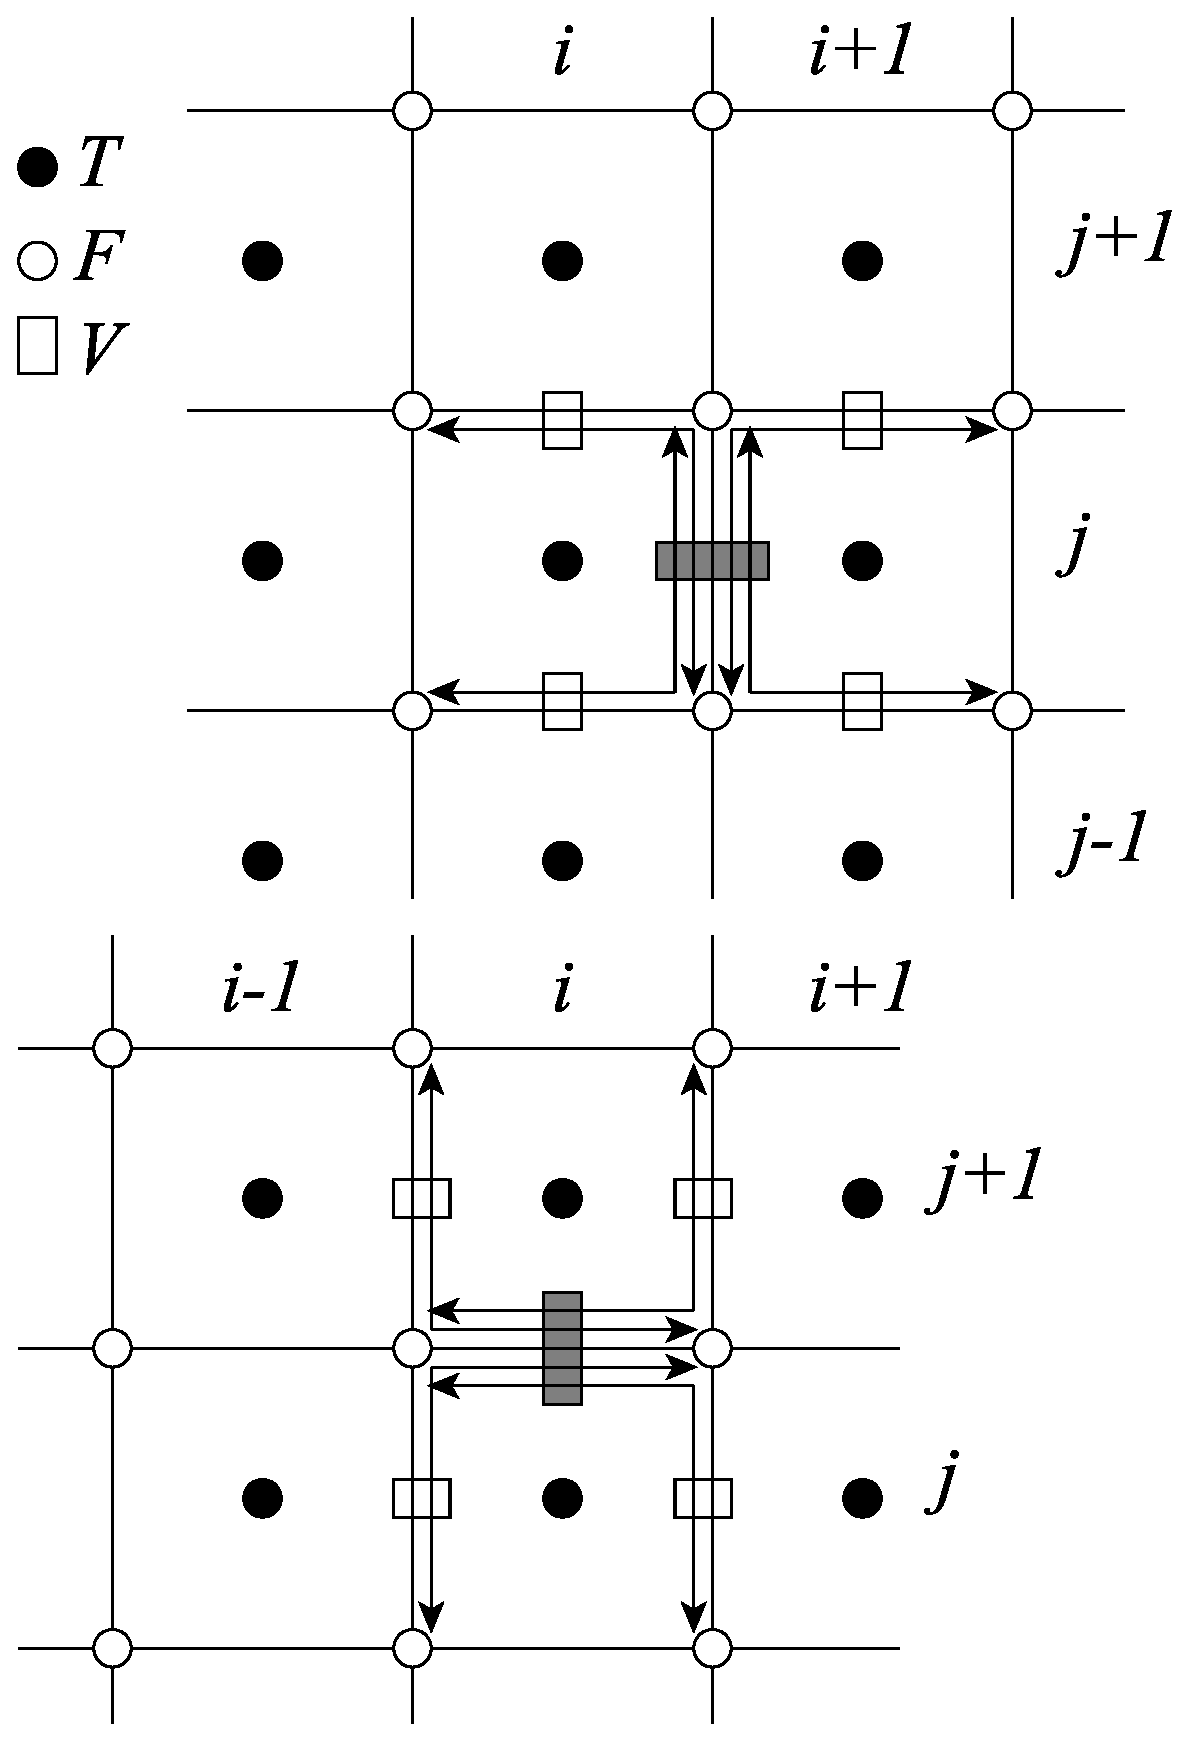
\includegraphics[width=0.70\textwidth]{Fig_DYN_een_triad}
\caption{ \protect\label{fig:DYN_een_triad}
  Triads used in the energy and enstrophy conserving scheme (een) for
  $u$-component (upper panel) and $v$-component (lower panel).}
\end{center}   \end{figure}
%>>>>>>>>>>>>>>>>>>>>>>>>>>>>>>>>

A key point in \autoref{eq:een_e3f} is how the averaging in the \textbf{i}- and \textbf{j}- directions is made. 
It uses the sum of masked t-point vertical scale factor divided either by the sum of the four t-point masks
(\np{nn\_een\_e3f}\forcode{ = 1}), or just by $4$ (\np{nn\_een\_e3f}\forcode{ = .true.}).
The latter case preserves the continuity of $e_{3f}$ when one or more of the neighbouring $e_{3t}$ tends to zero and
extends by continuity the value of $e_{3f}$ into the land areas.
This case introduces a sub-grid-scale topography at f-points
(with a systematic reduction of $e_{3f}$ when a model level intercept the bathymetry)
that tends to reinforce the topostrophy of the flow
($i.e.$ the tendency of the flow to follow the isobaths) \citep{Penduff_al_OS07}. 

Next, the vorticity triads, $ {^i_j}\mathbb{Q}^{i_p}_{j_p}$ can be defined at a $T$-point as
the following triad combinations of the neighbouring potential vorticities defined at f-points
(\autoref{fig:DYN_een_triad}): 
\begin{equation} \label{eq:Q_triads}
_i^j \mathbb{Q}^{i_p}_{j_p}
= \frac{1}{12} \ \left(   q^{i-i_p}_{j+j_p} + q^{i+j_p}_{j+i_p} + q^{i+i_p}_{j-j_p}  \right)
\end{equation}
where the indices $i_p$ and $k_p$ take the values: $i_p = -1/2$ or $1/2$ and $j_p = -1/2$ or $1/2$. 

Finally, the vorticity terms are represented as: 
\begin{equation} \label{eq:dynvor_een}
\left\{ {
\begin{aligned}
 +q\,e_3 \, v 	&\equiv +\frac{1}{e_{1u} }   \sum_{\substack{i_p,\,k_p}} 
                         {^{i+1/2-i_p}_j}  \mathbb{Q}^{i_p}_{j_p}  \left( e_{1v}\,e_{3v} \;v  \right)^{i+1/2-i_p}_{j+j_p}   \\
 - q\,e_3 \, u     &\equiv -\frac{1}{e_{2v} }    \sum_{\substack{i_p,\,k_p}} 
                         {^i_{j+1/2-j_p}}  \mathbb{Q}^{i_p}_{j_p}  \left( e_{2u}\,e_{3u} \;u  \right)^{i+i_p}_{j+1/2-j_p}   \\
\end{aligned} 
} \right.
\end{equation} 

This EEN scheme in fact combines the conservation properties of the ENS and ENE schemes.
It conserves both total energy and potential enstrophy in the limit of horizontally nondivergent flow
($i.e.$ $\chi$=$0$) (see \autoref{subsec:C_vorEEN}). 
Applied to a realistic ocean configuration, it has been shown that it leads to a significant reduction of
the noise in the vertical velocity field \citep{Le_Sommer_al_OM09}.
Furthermore, used in combination with a partial steps representation of bottom topography,
it improves the interaction between current and topography,
leading to a larger topostrophy of the flow \citep{Barnier_al_OD06, Penduff_al_OS07}. 

%--------------------------------------------------------------------------------------------------------------
%           Kinetic Energy Gradient term
%--------------------------------------------------------------------------------------------------------------
\subsection{Kinetic energy gradient term (\protect\mdl{dynkeg})}
\label{subsec:DYN_keg}

As demonstrated in \autoref{apdx:C},
there is a single discrete formulation of the kinetic energy gradient term that,
together with the formulation chosen for the vertical advection (see below),
conserves the total kinetic energy:
\begin{equation} \label{eq:dynkeg}
\left\{ \begin{aligned}
 -\frac{1}{2 \; e_{1u} }  & \ \delta _{i+1/2} \left[ {\overline {u^2}^{\,i} + \overline{v^2}^{\,j}} \right]   \\
 -\frac{1}{2 \; e_{2v} }  & \ \delta _{j+1/2} \left[ {\overline {u^2}^{\,i} + \overline{v^2}^{\,j}} \right]    
\end{aligned} \right.
\end{equation} 

%--------------------------------------------------------------------------------------------------------------
%           Vertical advection term
%--------------------------------------------------------------------------------------------------------------
\subsection{Vertical advection term (\protect\mdl{dynzad}) }
\label{subsec:DYN_zad}

The discrete formulation of the vertical advection, t
ogether with the formulation chosen for the gradient of kinetic energy (KE) term,
conserves the total kinetic energy.
Indeed, the change of KE due to the vertical advection is exactly balanced by
the change of KE due to the gradient of KE (see \autoref{apdx:C}).
\begin{equation} \label{eq:dynzad}
\left\{ 		\begin{aligned}
-\frac{1} {e_{1u}\,e_{2u}\,e_{3u}} &\ \overline{\ \overline{ e_{1t}\,e_{2t}\;w } ^{\,i+1/2}  \;\delta _{k+1/2} \left[ u \right]\  }^{\,k}  \\
-\frac{1} {e_{1v}\,e_{2v}\,e_{3v}}  &\ \overline{\ \overline{ e_{1t}\,e_{2t}\;w } ^{\,j+1/2}  \;\delta _{k+1/2} \left[ u \right]\  }^{\,k} 
\end{aligned}         \right.
\end{equation} 
When \np{ln\_dynzad\_zts}\forcode{ = .true.},
a split-explicit time stepping with 5 sub-timesteps is used on the vertical advection term.
This option can be useful when the value of the timestep is limited by vertical advection \citep{Lemarie_OM2015}. 
Note that in this case,
a similar split-explicit time stepping should be used on vertical advection of tracer to ensure a better stability,
an option which is only available with a TVD scheme (see \np{ln\_traadv\_tvd\_zts} in \autoref{subsec:TRA_adv_tvd}).


% ================================================================
% Coriolis and Advection : flux form
% ================================================================
\section{Coriolis and advection: flux form}
\label{sec:DYN_adv_cor_flux}
%------------------------------------------nam_dynadv----------------------------------------------------

\nlst{namdyn_adv} 
%-------------------------------------------------------------------------------------------------------------

Options are defined through the \ngn{namdyn\_adv} namelist variables.
In the flux form (as in the vector invariant form),
the Coriolis and momentum advection terms are evaluated using a leapfrog scheme,
$i.e.$ the velocity appearing in their expressions is centred in time (\textit{now} velocity).
At the lateral boundaries either free slip,
no slip or partial slip boundary conditions are applied following \autoref{chap:LBC}.


%--------------------------------------------------------------------------------------------------------------
%           Coriolis plus curvature metric terms
%--------------------------------------------------------------------------------------------------------------
\subsection{Coriolis plus curvature metric terms (\protect\mdl{dynvor}) }
\label{subsec:DYN_cor_flux}

In flux form, the vorticity term reduces to a Coriolis term in which the Coriolis parameter has been modified to account for the "metric" term.
This altered Coriolis parameter is thus discretised at $f$-points.
It is given by: 
\begin{multline} \label{eq:dyncor_metric}
f+\frac{1}{e_1 e_2 }\left( {v\frac{\partial e_2 }{\partial i}  -  u\frac{\partial e_1 }{\partial j}} \right)  \\
   \equiv   f + \frac{1}{e_{1f} e_{2f} } \left( { \ \overline v ^{i+1/2}\delta _{i+1/2} \left[ {e_{2u} } \right]  
                                                                 -  \overline u ^{j+1/2}\delta _{j+1/2} \left[ {e_{1u} } \right]  }  \ \right)
\end{multline} 

Any of the (\autoref{eq:dynvor_ens}), (\autoref{eq:dynvor_ene}) and (\autoref{eq:dynvor_een}) schemes can be used to
compute the product of the Coriolis parameter and the vorticity.
However, the energy-conserving scheme (\autoref{eq:dynvor_een}) has exclusively been used to date.
This term is evaluated using a leapfrog scheme, $i.e.$ the velocity is centred in time (\textit{now} velocity).

%--------------------------------------------------------------------------------------------------------------
%           Flux form Advection term
%--------------------------------------------------------------------------------------------------------------
\subsection{Flux form advection term (\protect\mdl{dynadv}) }
\label{subsec:DYN_adv_flux}

The discrete expression of the advection term is given by:
\begin{equation} \label{eq:dynadv}
\left\{ 
\begin{aligned}
\frac{1}{e_{1u}\,e_{2u}\,e_{3u}} 
\left(      \delta _{i+1/2} \left[ \overline{e_{2u}\,e_{3u}\;u }^{i       }  \ u_t      \right]    
          + \delta _{j       } \left[ \overline{e_{1u}\,e_{3u}\;v }^{i+1/2}  \ u_f      \right] \right.  \ \;   \\
\left.   + \delta _{k      } \left[ \overline{e_{1w}\,e_{2w}\;w}^{i+1/2}  \ u_{uw} \right] \right)   \\
\\
\frac{1}{e_{1v}\,e_{2v}\,e_{3v}} 
\left(     \delta _{i       } \left[ \overline{e_{2u}\,e_{3u }\;u }^{j+1/2} \ v_f       \right] 
         + \delta _{j+1/2} \left[ \overline{e_{1u}\,e_{3u }\;v }^{i       } \ v_t       \right] \right.  \ \, \, \\
\left.  + \delta _{k      } \left[ \overline{e_{1w}\,e_{2w}\;w}^{j+1/2} \ v_{vw}  \right] \right) \\
\end{aligned}
\right.
\end{equation}

Two advection schemes are available:
a $2^{nd}$ order centered finite difference scheme, CEN2,
or a $3^{rd}$ order upstream biased scheme, UBS.
The latter is described in \citet{Shchepetkin_McWilliams_OM05}.
The schemes are selected using the namelist logicals \np{ln\_dynadv\_cen2} and \np{ln\_dynadv\_ubs}. 
In flux form, the schemes differ by the choice of a space and time interpolation to define the value of
$u$ and $v$ at the centre of each face of $u$- and $v$-cells, $i.e.$ at the $T$-, $f$-,
and $uw$-points for $u$ and at the $f$-, $T$- and $vw$-points for $v$. 

%-------------------------------------------------------------
%                 2nd order centred scheme
%-------------------------------------------------------------
\subsubsection{CEN2: $2^{nd}$ order centred scheme (\protect\np{ln\_dynadv\_cen2}\forcode{ = .true.})}
\label{subsec:DYN_adv_cen2}

In the centered $2^{nd}$ order formulation, the velocity is evaluated as the mean of the two neighbouring points:
\begin{equation} \label{eq:dynadv_cen2}
\left\{ 		\begin{aligned}
 u_T^{cen2} &=\overline u^{i }       \quad &  u_F^{cen2} &=\overline u^{j+1/2}  \quad &  u_{uw}^{cen2} &=\overline u^{k+1/2}   \\
 v_F^{cen2} &=\overline v ^{i+1/2} \quad & v_F^{cen2} &=\overline v^j		\quad &  v_{vw}^{cen2} &=\overline v ^{k+1/2}  \\
\end{aligned}      \right.
\end{equation} 

The scheme is non diffusive (i.e. conserves the kinetic energy) but dispersive ($i.e.$ it may create false extrema).
It is therefore notoriously noisy and must be used in conjunction with an explicit diffusion operator to
produce a sensible solution.
The associated time-stepping is performed using a leapfrog scheme in conjunction with an Asselin time-filter,
so $u$ and $v$ are the \emph{now} velocities.

%-------------------------------------------------------------
%                 UBS scheme
%-------------------------------------------------------------
\subsubsection{UBS: Upstream Biased Scheme (\protect\np{ln\_dynadv\_ubs}\forcode{ = .true.})}
\label{subsec:DYN_adv_ubs}

The UBS advection scheme is an upstream biased third order scheme based on
an upstream-biased parabolic interpolation.
For example, the evaluation of $u_T^{ubs} $ is done as follows:
\begin{equation} \label{eq:dynadv_ubs}
u_T^{ubs} =\overline u ^i-\;\frac{1}{6} 	\begin{cases}
		u"_{i-1/2}& 	\text{if $\ \overline{e_{2u}\,e_{3u} \ u}^i  \geqslant 0$ } 	\\
		u"_{i+1/2}& 	\text{if $\ \overline{e_{2u}\,e_{3u} \ u}^i  < 0$ }
\end{cases}
\end{equation}
where $u"_{i+1/2} =\delta _{i+1/2} \left[ {\delta _i \left[ u \right]} \right]$.
This results in a dissipatively dominant ($i.e.$ hyper-diffusive) truncation error
\citep{Shchepetkin_McWilliams_OM05}.
The overall performance of the advection scheme is similar to that reported in \citet{Farrow1995}.
It is a relatively good compromise between accuracy and smoothness.
It is not a \emph{positive} scheme, meaning that false extrema are permitted.
But the amplitudes of the false extrema are significantly reduced over those in the centred second order method.
As the scheme already includes a diffusion component, it can be used without explicit lateral diffusion on momentum 
($i.e.$ \np{ln\_dynldf\_lap}\forcode{ = }\np{ln\_dynldf\_bilap}\forcode{ = .false.}),
and it is recommended to do so.

The UBS scheme is not used in all directions.
In the vertical, the centred $2^{nd}$ order evaluation of the advection is preferred, $i.e.$ $u_{uw}^{ubs}$ and
$u_{vw}^{ubs}$ in \autoref{eq:dynadv_cen2} are used.
UBS is diffusive and is associated with vertical mixing of momentum. \gmcomment{ gm  pursue the 
sentence:Since vertical mixing of momentum is a source term of the TKE equation...  }

For stability reasons, the first term in (\autoref{eq:dynadv_ubs}),
which corresponds to a second order centred scheme, is evaluated using the \textit{now} velocity (centred in time),
while the second term, which is the diffusion part of the scheme,
is evaluated using the \textit{before} velocity (forward in time).
This is discussed by \citet{Webb_al_JAOT98} in the context of the Quick advection scheme.

Note that the UBS and QUICK (Quadratic Upstream Interpolation for Convective Kinematics) schemes only differ by
one coefficient.
Replacing $1/6$ by $1/8$ in (\autoref{eq:dynadv_ubs}) leads to the QUICK advection scheme \citep{Webb_al_JAOT98}.
This option is not available through a namelist parameter, since the $1/6$ coefficient is hard coded.
Nevertheless it is quite easy to make the substitution in the \mdl{dynadv\_ubs} module and obtain a QUICK scheme.

Note also that in the current version of \mdl{dynadv\_ubs},
there is also the possibility of using a $4^{th}$ order evaluation of the advective velocity as in ROMS.
This is an error and should be suppressed soon.
%%%
\gmcomment{action :  this have to be done}
%%%

% ================================================================
%           Hydrostatic pressure gradient term
% ================================================================
\section{Hydrostatic pressure gradient (\protect\mdl{dynhpg})}
\label{sec:DYN_hpg}
%------------------------------------------nam_dynhpg---------------------------------------------------

\nlst{namdyn_hpg} 
%-------------------------------------------------------------------------------------------------------------

Options are defined through the \ngn{namdyn\_hpg} namelist variables.
The key distinction between the different algorithms used for
the hydrostatic pressure gradient is the vertical coordinate used,
since HPG is a \emph{horizontal} pressure gradient, $i.e.$ computed along geopotential surfaces.
As a result, any tilt of the surface of the computational levels will require a specific treatment to
compute the hydrostatic pressure gradient.

The hydrostatic pressure gradient term is evaluated either using a leapfrog scheme,
$i.e.$ the density appearing in its expression is centred in time (\emph{now} $\rho$),
or a semi-implcit scheme.
At the lateral boundaries either free slip, no slip or partial slip boundary conditions are applied.

%--------------------------------------------------------------------------------------------------------------
%           z-coordinate with full step
%--------------------------------------------------------------------------------------------------------------
\subsection{Full step $Z$-coordinate (\protect\np{ln\_dynhpg\_zco}\forcode{ = .true.})}
\label{subsec:DYN_hpg_zco}

The hydrostatic pressure can be obtained by integrating the hydrostatic equation vertically from the surface.
However, the pressure is large at great depth while its horizontal gradient is several orders of magnitude smaller.
This may lead to large truncation errors in the pressure gradient terms.
Thus, the two horizontal components of the hydrostatic pressure gradient are computed directly as follows:

for $k=km$ (surface layer, $jk=1$ in the code)
\begin{equation} \label{eq:dynhpg_zco_surf}
\left\{ \begin{aligned}
					\left. \delta _{i+1/2} \left[  p^h 			 \right] \right|_{k=km} 
&= \frac{1}{2} g \ 	\left. \delta _{i+1/2} \left[  e_{3w} \ \rho \right] \right|_{k=km}   \\
     					\left. \delta _{j+1/2} \left[  p^h  			 \right] \right|_{k=km} 
&= \frac{1}{2} g \ 	\left. \delta _{j+1/2} \left[  e_{3w} \ \rho \right] \right|_{k=km}   \\
\end{aligned} \right.
\end{equation} 

for $1<k<km$ (interior layer)
\begin{equation} \label{eq:dynhpg_zco}
\left\{ \begin{aligned}
					\left. \delta _{i+1/2} \left[  p^h 			 \right] \right|_{k} 
&=					\left. \delta _{i+1/2} \left[  p^h 			 \right] \right|_{k-1} 
+    \frac{1}{2}\;g\;	\left. \delta _{i+1/2} \left[  e_{3w} \ \overline {\rho}^{k+1/2} \right] \right|_{k}   \\
     					\left. \delta _{j+1/2} \left[  p^h  			 \right] \right|_{k} 
&=     				\left. \delta _{j+1/2} \left[  p^h  			 \right] \right|_{k-1} 
+    \frac{1}{2}\;g\;	\left. \delta _{j+1/2} \left[  e_{3w} \ \overline {\rho}^{k+1/2} \right] \right|_{k}   \\
\end{aligned} \right.
\end{equation} 

Note that the $1/2$ factor in (\autoref{eq:dynhpg_zco_surf}) is adequate because of the definition of $e_{3w}$ as
the vertical derivative of the scale factor at the surface level ($z=0$).
Note also that in case of variable volume level (\key{vvl} defined),
the surface pressure gradient is included in \autoref{eq:dynhpg_zco_surf} and
\autoref{eq:dynhpg_zco} through the space and time variations of the vertical scale factor $e_{3w}$.

%--------------------------------------------------------------------------------------------------------------
%           z-coordinate with partial step
%--------------------------------------------------------------------------------------------------------------
\subsection{Partial step $Z$-coordinate (\protect\np{ln\_dynhpg\_zps}\forcode{ = .true.})}
\label{subsec:DYN_hpg_zps}

With partial bottom cells, tracers in horizontally adjacent cells generally live at different depths.
Before taking horizontal gradients between these tracer points,
a linear interpolation is used to approximate the deeper tracer as if
it actually lived at the depth of the shallower tracer point. 

Apart from this modification,
the horizontal hydrostatic pressure gradient evaluated in the $z$-coordinate with partial step is exactly as in
the pure $z$-coordinate case.
As explained in detail in section \autoref{sec:TRA_zpshde},
the nonlinearity of pressure effects in the equation of state is such that
it is better to interpolate temperature and salinity vertically before computing the density.
Horizontal gradients of temperature and salinity are needed for the TRA modules,
which is the reason why the horizontal gradients of density at the deepest model level are computed in
module \mdl{zpsdhe} located in the TRA directory and described in \autoref{sec:TRA_zpshde}.

%--------------------------------------------------------------------------------------------------------------
%           s- and s-z-coordinates
%--------------------------------------------------------------------------------------------------------------
\subsection{$S$- and $Z$-$S$-coordinates}
\label{subsec:DYN_hpg_sco}

Pressure gradient formulations in an $s$-coordinate have been the subject of a vast number of papers
($e.g.$, \citet{Song1998, Shchepetkin_McWilliams_OM05}). 
A number of different pressure gradient options are coded but the ROMS-like,
density Jacobian with cubic polynomial method is currently disabled whilst known bugs are under investigation.

$\bullet$ Traditional coding (see for example \citet{Madec_al_JPO96}: (\np{ln\_dynhpg\_sco}\forcode{ = .true.})
\begin{equation} \label{eq:dynhpg_sco}
\left\{ \begin{aligned}
 - \frac{1}    					{\rho_o \, e_{1u}} \;	\delta _{i+1/2} \left[  p^h  \right] 
+ \frac{g\; \overline {\rho}^{i+1/2}}	{\rho_o \, e_{1u}} \;	\delta _{i+1/2} \left[  z_t   \right]    \\
 - \frac{1}    					{\rho_o \, e_{2v}} \;	\delta _{j+1/2} \left[  p^h  \right]  
+ \frac{g\; \overline {\rho}^{j+1/2}}	{\rho_o \, e_{2v}} \;	\delta _{j+1/2} \left[  z_t   \right]    \\
\end{aligned} \right.
\end{equation} 

Where the first term is the pressure gradient along coordinates,
computed as in \autoref{eq:dynhpg_zco_surf} - \autoref{eq:dynhpg_zco},
and $z_T$ is the depth of the $T$-point evaluated from the sum of the vertical scale factors at the $w$-point 
($e_{3w}$).
 
$\bullet$ Traditional coding with adaptation for ice shelf cavities (\np{ln\_dynhpg\_isf}\forcode{ = .true.}).
This scheme need the activation of ice shelf cavities (\np{ln\_isfcav}\forcode{ = .true.}).

$\bullet$ Pressure Jacobian scheme (prj) (a research paper in preparation) (\np{ln\_dynhpg\_prj}\forcode{ = .true.})

$\bullet$ Density Jacobian with cubic polynomial scheme (DJC) \citep{Shchepetkin_McWilliams_OM05} 
(\np{ln\_dynhpg\_djc}\forcode{ = .true.}) (currently disabled; under development)

Note that expression \autoref{eq:dynhpg_sco} is commonly used when the variable volume formulation is activated
(\key{vvl}) because in that case, even with a flat bottom,
the coordinate surfaces are not horizontal but follow the free surface \citep{Levier2007}.
The pressure jacobian scheme (\np{ln\_dynhpg\_prj}\forcode{ = .true.}) is available as
an improved option to \np{ln\_dynhpg\_sco}\forcode{ = .true.} when \key{vvl} is active.
The pressure Jacobian scheme uses a constrained cubic spline to
reconstruct the density profile across the water column.
This method maintains the monotonicity between the density nodes.
The pressure can be calculated by analytical integration of the density profile and
a pressure Jacobian method is used to solve the horizontal pressure gradient.
This method can provide a more accurate calculation of the horizontal pressure gradient than the standard scheme.

\subsection{Ice shelf cavity}
\label{subsec:DYN_hpg_isf}
Beneath an ice shelf, the total pressure gradient is the sum of the pressure gradient due to the ice shelf load and
the pressure gradient due to the ocean load.
If cavity opened (\np{ln\_isfcav}\forcode{ = .true.}) these 2 terms can be calculated by
setting \np{ln\_dynhpg\_isf}\forcode{ = .true.}.
No other scheme are working with the ice shelf.\\

$\bullet$ The main hypothesis to compute the ice shelf load is that the ice shelf is in an isostatic equilibrium.
The top pressure is computed integrating from surface to the base of the ice shelf a reference density profile
(prescribed as density of a water at 34.4 PSU and -1.9\degC) and
corresponds to the water replaced by the ice shelf.
This top pressure is constant over time.
A detailed description of this method is described in \citet{Losch2008}.\\

$\bullet$ The ocean load is computed using the expression \autoref{eq:dynhpg_sco} described in
\autoref{subsec:DYN_hpg_sco}. 

%--------------------------------------------------------------------------------------------------------------
%           Time-scheme
%--------------------------------------------------------------------------------------------------------------
\subsection{Time-scheme (\protect\np{ln\_dynhpg\_imp}\forcode{ = .true./.false.})}
\label{subsec:DYN_hpg_imp}

The default time differencing scheme used for the horizontal pressure gradient is a leapfrog scheme and
therefore the density used in all discrete expressions given above is the  \textit{now} density,
computed from the \textit{now} temperature and salinity.
In some specific cases
(usually high resolution simulations over an ocean domain which includes weakly stratified regions)
the physical phenomenon that controls the time-step is internal gravity waves (IGWs).
A semi-implicit scheme for doubling the stability limit associated with IGWs can be used
\citep{Brown_Campana_MWR78, Maltrud1998}.
It involves the evaluation of the hydrostatic pressure gradient as
an average over the three time levels $t-\rdt$, $t$, and $t+\rdt$
($i.e.$  \textit{before},  \textit{now} and  \textit{after} time-steps),
rather than at the central time level $t$ only, as in the standard leapfrog scheme. 

$\bullet$ leapfrog scheme (\np{ln\_dynhpg\_imp}\forcode{ = .true.}):

\begin{equation} \label{eq:dynhpg_lf}
\frac{u^{t+\rdt}-u^{t-\rdt}}{2\rdt} = \;\cdots \;
	-\frac{1}{\rho _o \,e_{1u} }\delta _{i+1/2} \left[ {p_h^t } \right]
\end{equation}

$\bullet$ semi-implicit scheme (\np{ln\_dynhpg\_imp}\forcode{ = .true.}):
\begin{equation} \label{eq:dynhpg_imp}
\frac{u^{t+\rdt}-u^{t-\rdt}}{2\rdt} = \;\cdots \;
	-\frac{1}{4\,\rho _o \,e_{1u} } \delta_{i+1/2} \left[ p_h^{t+\rdt} +2\,p_h^t +p_h^{t-\rdt}  \right]
\end{equation}

The semi-implicit time scheme \autoref{eq:dynhpg_imp} is made possible without
significant additional computation since the density can be updated to time level $t+\rdt$ before
computing the horizontal hydrostatic pressure gradient.
It can be easily shown that the stability limit associated with the hydrostatic pressure gradient doubles using
\autoref{eq:dynhpg_imp} compared to that using the standard leapfrog scheme \autoref{eq:dynhpg_lf}.
Note that \autoref{eq:dynhpg_imp} is equivalent to applying a time filter to the pressure gradient to
eliminate high frequency IGWs.
Obviously, when using \autoref{eq:dynhpg_imp},
the doubling of the time-step is achievable only if no other factors control the time-step,
such as the stability limits associated with advection or diffusion.

In practice, the semi-implicit scheme is used when \np{ln\_dynhpg\_imp}\forcode{ = .true.}.
In this case, we choose to apply the time filter to temperature and salinity used in the equation of state,
instead of applying it to the hydrostatic pressure or to the density,
so that no additional storage array has to be defined.
The density used to compute the hydrostatic pressure gradient (whatever the formulation) is evaluated as follows:
\begin{equation} \label{eq:rho_flt}
	\rho^t = \rho( \widetilde{T},\widetilde {S},z_t)
 \quad	  \text{with}	\quad 
	\widetilde{X} = 1 / 4 \left(  X^{t+\rdt} +2 \,X^t + X^{t-\rdt}  \right)
\end{equation}

Note that in the semi-implicit case, it is necessary to save the filtered density,
an extra three-dimensional field, in the restart file to restart the model with exact reproducibility.
This option is controlled by  \np{nn\_dynhpg\_rst}, a namelist parameter.

% ================================================================
% Surface Pressure Gradient
% ================================================================
\section{Surface pressure gradient (\protect\mdl{dynspg})}
\label{sec:DYN_spg}
%-----------------------------------------nam_dynspg----------------------------------------------------

\nlst{namdyn_spg} 
%------------------------------------------------------------------------------------------------------------

$\ $\newline      %force an empty line

Options are defined through the \ngn{namdyn\_spg} namelist variables.
The surface pressure gradient term is related to the representation of the free surface (\autoref{sec:PE_hor_pg}).
The main distinction is between the fixed volume case (linear free surface) and
the variable volume case (nonlinear free surface, \key{vvl} is defined).
In the linear free surface case (\autoref{subsec:PE_free_surface})
the vertical scale factors $e_{3}$ are fixed in time,
while they are time-dependent in the nonlinear case (\autoref{subsec:PE_free_surface}).
With both linear and nonlinear free surface, external gravity waves are allowed in the equations, 
which imposes a very small time step when an explicit time stepping is used.
Two methods are proposed to allow a longer time step for the three-dimensional equations: 
the filtered free surface, which is a modification of the continuous equations (see \autoref{eq:PE_flt}), 
and the split-explicit free surface described below.
The extra term introduced in the filtered method is calculated implicitly, 
so that the update of the next velocities is done in module \mdl{dynspg\_flt} and not in \mdl{dynnxt}.


The form of the surface pressure gradient term depends on how the user wants to
handle the fast external gravity waves that are a solution of the analytical equation (\autoref{sec:PE_hor_pg}).
Three formulations are available, all controlled by a CPP key (ln\_dynspg\_xxx):
an explicit formulation which requires a small time step;
a filtered free surface formulation which allows a larger time step by
adding a filtering term into the momentum equation; 
and a split-explicit free surface formulation, described below, which also allows a larger time step.

The extra term introduced in the filtered method is calculated implicitly, so that a solver is used to compute it.
As a consequence the update of the $next$ velocities is done in module \mdl{dynspg\_flt} and not in \mdl{dynnxt}.


%--------------------------------------------------------------------------------------------------------------
% Explicit free surface formulation
%--------------------------------------------------------------------------------------------------------------
\subsection{Explicit free surface (\protect\key{dynspg\_exp})}
\label{subsec:DYN_spg_exp}

In the explicit free surface formulation (\key{dynspg\_exp} defined),
the model time step is chosen to be small enough to resolve the external gravity waves
(typically a few tens of seconds).
The surface pressure gradient, evaluated using a leap-frog scheme ($i.e.$ centered in time),
is thus simply given by :
\begin{equation} \label{eq:dynspg_exp}
\left\{ \begin{aligned}
 - \frac{1}{e_{1u}\,\rho_o} \;	\delta _{i+1/2} \left[  \,\rho \,\eta\,  \right] 	\\
 - \frac{1}{e_{2v}\,\rho_o} \;	\delta _{j+1/2} \left[  \,\rho \,\eta\,  \right]  
\end{aligned} \right.
\end{equation} 

Note that in the non-linear free surface case ($i.e.$ \key{vvl} defined),
the surface pressure gradient is already included in the momentum tendency through
the level thickness variation allowed in the computation of the hydrostatic pressure gradient.
Thus, nothing is done in the \mdl{dynspg\_exp} module.

%--------------------------------------------------------------------------------------------------------------
% Split-explict free surface formulation
%--------------------------------------------------------------------------------------------------------------
\subsection{Split-explicit free surface (\protect\key{dynspg\_ts})}
\label{subsec:DYN_spg_ts}
%------------------------------------------namsplit-----------------------------------------------------------
%
%\nlst{namsplit}
%-------------------------------------------------------------------------------------------------------------

The split-explicit free surface formulation used in \NEMO (\key{dynspg\_ts} defined),
also called the time-splitting formulation, follows the one proposed by \citet{Shchepetkin_McWilliams_OM05}.
The general idea is to solve the free surface equation and the associated barotropic velocity equations with
a smaller time step than $\rdt$, the time step used for the three dimensional prognostic variables
(\autoref{fig:DYN_dynspg_ts}).
The size of the small time step, $\rdt_e$ (the external mode or barotropic time step) is provided through
the \np{nn\_baro} namelist parameter as: $\rdt_e = \rdt / nn\_baro$.
This parameter can be optionally defined automatically (\np{ln\_bt\_nn\_auto}\forcode{ = .true.}) considering that
the stability of the barotropic system is essentially controled by external waves propagation.
Maximum Courant number is in that case time independent, and easily computed online from the input bathymetry.
Therefore, $\rdt_e$ is adjusted so that the Maximum allowed Courant number is smaller than \np{rn\_bt\_cmax}.

%%%
The barotropic mode solves the following equations:
\begin{subequations} \label{eq:BT}
  \begin{equation}     \label{eq:BT_dyn}
\frac{\partial {\rm \overline{{\bf U}}_h} }{\partial t}=
 -f\;{\rm {\bf k}}\times {\rm \overline{{\bf U}}_h} 
-g\nabla _h \eta -\frac{c_b^{\textbf U}}{H+\eta} \rm {\overline{{\bf U}}_h} + \rm {\overline{\bf G}}
  \end{equation}

  \begin{equation} \label{eq:BT_ssh}
\frac{\partial \eta }{\partial t}=-\nabla \cdot \left[ {\left( {H+\eta } \right) \; {\rm{\bf \overline{U}}}_h \,} \right]+P-E
  \end{equation}
\end{subequations}
where $\rm {\overline{\bf G}}$ is a forcing term held constant, containing coupling term between modes,
surface atmospheric forcing as well as slowly varying barotropic terms not explicitly computed to gain efficiency.
The third term on the right hand side of \autoref{eq:BT_dyn} represents the bottom stress
(see section \autoref{sec:ZDF_bfr}), explicitly accounted for at each barotropic iteration.
Temporal discretization of the system above follows a three-time step Generalized Forward Backward algorithm
detailed in \citet{Shchepetkin_McWilliams_OM05}.
AB3-AM4 coefficients used in \NEMO follow the second-order accurate,
"multi-purpose" stability compromise as defined in \citet{Shchepetkin_McWilliams_Bk08}
(see their figure 12, lower left). 

%>   >   >   >   >   >   >   >   >   >   >   >   >   >   >   >   >   >   >   >   >   >   >   >   >   >   >   >
\begin{figure}[!t]    \begin{center}
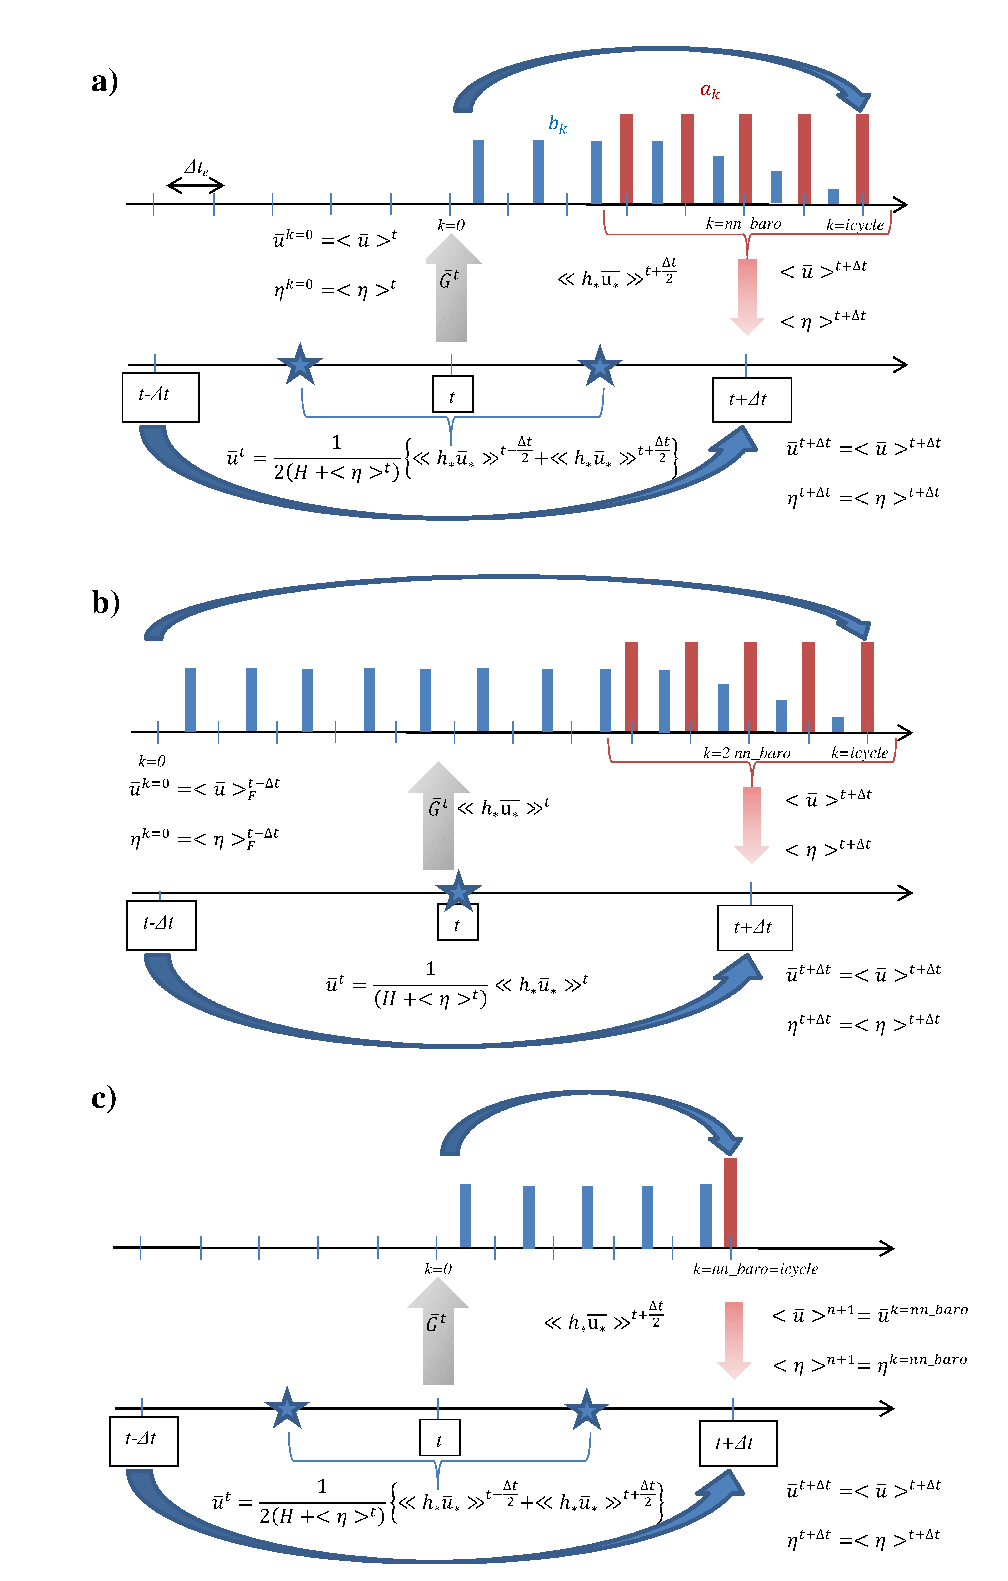
\includegraphics[width=0.7\textwidth]{Fig_DYN_dynspg_ts}
\caption{  \protect\label{fig:DYN_dynspg_ts}
  Schematic of the split-explicit time stepping scheme for the external and internal modes.
  Time increases to the right. In this particular exemple,
  a boxcar averaging window over $nn\_baro$ barotropic time steps is used ($nn\_bt\_flt=1$) and $nn\_baro=5$.
  Internal mode time steps (which are also the model time steps) are denoted by $t-\rdt$, $t$ and $t+\rdt$.
  Variables with $k$ superscript refer to instantaneous barotropic variables,
  $< >$ and $<< >>$ operator refer to time filtered variables using respectively primary (red vertical bars) and
  secondary weights (blue vertical bars).
  The former are used to obtain time filtered quantities at $t+\rdt$ while
  the latter are used to obtain time averaged transports to advect tracers.
  a) Forward time integration: \protect\np{ln\_bt\_fw}\forcode{ = .true.},
  \protect\np{ln\_bt\_av}\forcode{ = .true.}.
  b) Centred time integration: \protect\np{ln\_bt\_fw}\forcode{ = .false.},
  \protect\np{ln\_bt\_av}\forcode{ = .true.}.
  c) Forward time integration with no time filtering (POM-like scheme):
  \protect\np{ln\_bt\_fw}\forcode{ = .true.}, \protect\np{ln\_bt\_av}\forcode{ = .false.}. }
\end{center}    \end{figure}
%>   >   >   >   >   >   >   >   >   >   >   >   >   >   >   >   >   >   >   >   >   >   >   >   >   >   >   >

In the default case (\np{ln\_bt\_fw}\forcode{ = .true.}),
the external mode is integrated between \textit{now} and \textit{after} baroclinic time-steps
(\autoref{fig:DYN_dynspg_ts}a).
To avoid aliasing of fast barotropic motions into three dimensional equations,
time filtering is eventually applied on barotropic quantities (\np{ln\_bt\_av}\forcode{ = .true.}).
In that case, the integration is extended slightly beyond \textit{after} time step to
provide time filtered quantities.
These are used for the subsequent initialization of the barotropic mode in the following baroclinic step.
Since external mode equations written at baroclinic time steps finally follow a forward time stepping scheme, 
asselin filtering is not applied to barotropic quantities.\\
Alternatively, one can choose to integrate barotropic equations starting from \textit{before} time step
(\np{ln\_bt\_fw}\forcode{ = .false.}).
Although more computationaly expensive ( \np{nn\_baro} additional iterations are indeed necessary),
the baroclinic to barotropic forcing term given at \textit{now} time step become centred in
the middle of the integration window.
It can easily be shown that this property removes part of splitting errors between modes,
which increases the overall numerical robustness.
%references to Patrick Marsaleix' work here. Also work done by SHOM group.

%%%

As far as tracer conservation is concerned,
barotropic velocities used to advect tracers must also be updated at \textit{now} time step.
This implies to change the traditional order of computations in \NEMO:
most of momentum trends (including the barotropic mode calculation) updated first, tracers' after.
This \textit{de facto} makes semi-implicit hydrostatic pressure gradient
(see section \autoref{subsec:DYN_hpg_imp})
and time splitting not compatible.
Advective barotropic velocities are obtained by using a secondary set of filtering weights,
uniquely defined from the filter coefficients used for the time averaging (\citet{Shchepetkin_McWilliams_OM05}).
Consistency between the time averaged continuity equation and the time stepping of tracers is here the key to
obtain exact conservation.

%%%

One can eventually choose to feedback instantaneous values by not using any time filter
(\np{ln\_bt\_av}\forcode{ = .false.}). 
In that case, external mode equations are continuous in time,
$i.e.$ they are not re-initialized when starting a new sub-stepping sequence.
This is the method used so far in the POM model, the stability being maintained by
refreshing at (almost) each barotropic time step advection and horizontal diffusion terms.
Since the latter terms have not been added in \NEMO for computational efficiency,
removing time filtering is not recommended except for debugging purposes.
This may be used for instance to appreciate the damping effect of the standard formulation on
external gravity waves in idealized or weakly non-linear cases.
Although the damping is lower than for the filtered free surface,
it is still significant as shown by \citet{Levier2007} in the case of an analytical barotropic Kelvin wave.

%>>>>>===============
\gmcomment{               %%% copy from griffies Book 

\textbf{title: Time stepping the barotropic system }

Assume knowledge of the full velocity and tracer fields at baroclinic time $\tau$.
Hence, we can update the surface height and vertically integrated velocity with a leap-frog scheme using
the small barotropic time step $\rdt$.
We have 

\begin{equation} \label{eq:DYN_spg_ts_eta}
\eta^{(b)}(\tau,t_{n+1}) - \eta^{(b)}(\tau,t_{n+1}) (\tau,t_{n-1})
	= 2 \rdt \left[-\nabla \cdot \textbf{U}^{(b)}(\tau,t_n) + \text{EMP}_w(\tau) \right] 
\end{equation}
\begin{multline} \label{eq:DYN_spg_ts_u}
\textbf{U}^{(b)}(\tau,t_{n+1}) - \textbf{U}^{(b)}(\tau,t_{n-1})  \\
	= 2\rdt \left[ - f \textbf{k} \times \textbf{U}^{(b)}(\tau,t_{n}) 
	- H(\tau) \nabla p_s^{(b)}(\tau,t_{n}) +\textbf{M}(\tau) \right]
\end{multline}
\

In these equations, araised (b) denotes values of surface height and vertically integrated velocity updated with
the barotropic time steps.
The $\tau$ time label on $\eta^{(b)}$ and $U^{(b)}$ denotes the baroclinic time at which
the vertically integrated forcing $\textbf{M}(\tau)$
(note that this forcing includes the surface freshwater forcing),
the tracer fields, the freshwater flux $\text{EMP}_w(\tau)$,
and total depth of the ocean $H(\tau)$ are held for the duration of the barotropic time stepping over
a single cycle.
This is also the time that sets the barotropic time steps via 
\begin{equation} \label{eq:DYN_spg_ts_t}
t_n=\tau+n\rdt   
\end{equation}
with $n$ an integer.
The density scaled surface pressure is evaluated via 
\begin{equation} \label{eq:DYN_spg_ts_ps}
p_s^{(b)}(\tau,t_{n}) = \begin{cases}
	g \;\eta_s^{(b)}(\tau,t_{n}) \;\rho(\tau)_{k=1}) / \rho_o  &      \text{non-linear case} \\
	g \;\eta_s^{(b)}(\tau,t_{n})  &      \text{linear case} 
	\end{cases}
\end{equation}
To get started, we assume the following initial conditions 
\begin{equation} \label{eq:DYN_spg_ts_eta}
\begin{split}
\eta^{(b)}(\tau,t_{n=0}) &= \overline{\eta^{(b)}(\tau)}
\\
\eta^{(b)}(\tau,t_{n=1}) &= \eta^{(b)}(\tau,t_{n=0}) + \rdt \ \text{RHS}_{n=0} 
\end{split}
\end{equation}
with 
\begin{equation} \label{eq:DYN_spg_ts_etaF}
 \overline{\eta^{(b)}(\tau)} = \frac{1}{N+1} \sum\limits_{n=0}^N \eta^{(b)}(\tau-\rdt,t_{n})
\end{equation}
the time averaged surface height taken from the previous barotropic cycle.
Likewise, 
\begin{equation} \label{eq:DYN_spg_ts_u}
\textbf{U}^{(b)}(\tau,t_{n=0}) = \overline{\textbf{U}^{(b)}(\tau)}	\\
\\
\textbf{U}(\tau,t_{n=1}) = \textbf{U}^{(b)}(\tau,t_{n=0}) + \rdt \ \text{RHS}_{n=0}  	
\end{equation}
with 
\begin{equation} \label{eq:DYN_spg_ts_u}
 \overline{\textbf{U}^{(b)}(\tau)} 
 	= \frac{1}{N+1} \sum\limits_{n=0}^N\textbf{U}^{(b)}(\tau-\rdt,t_{n})
\end{equation}
the time averaged vertically integrated transport.
Notably, there is no Robert-Asselin time filter used in the barotropic portion of the integration. 

Upon reaching $t_{n=N} = \tau + 2\rdt \tau$ ,
the vertically integrated velocity is time averaged to produce the updated vertically integrated velocity at
baroclinic time $\tau + \rdt \tau$ 
\begin{equation} \label{eq:DYN_spg_ts_u}
\textbf{U}(\tau+\rdt) = \overline{\textbf{U}^{(b)}(\tau+\rdt)} 
 	= \frac{1}{N+1} \sum\limits_{n=0}^N\textbf{U}^{(b)}(\tau,t_{n})
\end{equation}
The surface height on the new baroclinic time step is then determined via a baroclinic leap-frog using
the following form 

\begin{equation} \label{eq:DYN_spg_ts_ssh}
\eta(\tau+\Delta) - \eta^{F}(\tau-\Delta) = 2\rdt \ \left[ - \nabla \cdot \textbf{U}(\tau) + \text{EMP}_w \right]  
\end{equation}

The use of this "big-leap-frog" scheme for the surface height ensures compatibility between
the mass/volume budgets and the tracer budgets.
More discussion of this point is provided in Chapter 10 (see in particular Section 10.2). 
 
In general, some form of time filter is needed to maintain integrity of the surface height field due to
the leap-frog splitting mode in equation \autoref{eq:DYN_spg_ts_ssh}.
We have tried various forms of such filtering,
with the following method discussed in \cite{Griffies_al_MWR01} chosen due to
its stability and reasonably good maintenance of tracer conservation properties (see ??).

\begin{equation} \label{eq:DYN_spg_ts_sshf}
\eta^{F}(\tau-\Delta) =  \overline{\eta^{(b)}(\tau)} 
\end{equation}
Another approach tried was 

\begin{equation} \label{eq:DYN_spg_ts_sshf2}
\eta^{F}(\tau-\Delta) = \eta(\tau) 
	+ (\alpha/2) \left[\overline{\eta^{(b)}}(\tau+\rdt)
				    + \overline{\eta^{(b)}}(\tau-\rdt) -2 \;\eta(\tau) \right]
\end{equation}

which is useful since it isolates all the time filtering aspects into the term multiplied by $\alpha$.
This isolation allows for an easy check that tracer conservation is exact when
eliminating tracer and surface height time filtering (see ?? for more complete discussion).
However, in the general case with a non-zero $\alpha$,
the filter \autoref{eq:DYN_spg_ts_sshf} was found to be more conservative, and so is recommended. 

}            %%end gm comment (copy of griffies book)

%>>>>>===============


%--------------------------------------------------------------------------------------------------------------
% Filtered free surface formulation
%--------------------------------------------------------------------------------------------------------------
\subsection{Filtered free surface (\protect\key{dynspg\_flt})}
\label{subsec:DYN_spg_fltp}

The filtered formulation follows the \citet{Roullet_Madec_JGR00} implementation. 
The extra term introduced in the equations (see \autoref{subsec:PE_free_surface}) is solved implicitly. 
The elliptic solvers available in the code are documented in \autoref{chap:MISC}.

%% gm %%======>>>>   given here the discrete eqs provided to the solver
\gmcomment{               %%% copy from chap-model basics 
\begin{equation} \label{eq:spg_flt}
\frac{\partial {\rm {\bf U}}_h }{\partial t}= {\rm {\bf M}}
- g \nabla \left( \tilde{\rho} \ \eta \right) 
- g \ T_c \nabla \left( \widetilde{\rho} \ \partial_t \eta \right) 
\end{equation}
where $T_c$, is a parameter with dimensions of time which characterizes the force, 
$\widetilde{\rho} = \rho / \rho_o$ is the dimensionless density,
and $\rm {\bf M}$ represents the collected contributions of the Coriolis, hydrostatic pressure gradient, 
non-linear and viscous terms in \autoref{eq:PE_dyn}.
}   %end gmcomment

Note that in the linear free surface formulation (\key{vvl} not defined),
the ocean depth is time-independent and so is the matrix to be inverted.
It is computed once and for all and applies to all ocean time steps. 

% ================================================================
% Lateral diffusion term
% ================================================================
\section{Lateral diffusion term and operators (\protect\mdl{dynldf})}
\label{sec:DYN_ldf}
%------------------------------------------nam_dynldf----------------------------------------------------

\nlst{namdyn_ldf} 
%-------------------------------------------------------------------------------------------------------------

Options are defined through the \ngn{namdyn\_ldf} namelist variables.
The options available for lateral diffusion are to use either laplacian (rotated or not) or biharmonic operators.
The coefficients may be constant or spatially variable;
the description of the coefficients is found in the chapter on lateral physics (\autoref{chap:LDF}).
The lateral diffusion of momentum is evaluated using a forward scheme,
$i.e.$ the velocity appearing in its expression is the \textit{before} velocity in time,
except for the pure vertical component that appears when a tensor of rotation is used.
This latter term is solved implicitly together with the vertical diffusion term (see \autoref{chap:STP}).

At the lateral boundaries either free slip,
no slip or partial slip boundary conditions are applied according to the user's choice (see \autoref{chap:LBC}).

\gmcomment{
  Hyperviscous operators are frequently used in the simulation of turbulent flows to
  control the dissipation of unresolved small scale features.
  Their primary role is to provide strong dissipation at the smallest scale supported by
  the grid while minimizing the impact on the larger scale features.
  Hyperviscous operators are thus designed to be more scale selective than the traditional,
  physically motivated Laplace operator.
  In finite difference methods,
  the biharmonic operator is frequently the method of choice to achieve this scale selective dissipation since
  its damping time ($i.e.$ its spin down time) scale like $\lambda^{-4}$ for disturbances of wavelength $\lambda$
  (so that short waves damped more rapidelly than long ones),
  whereas the Laplace operator damping time scales only like $\lambda^{-2}$.
}

% ================================================================
\subsection[Iso-level laplacian (\protect\np{ln\_dynldf\_lap}\forcode{ = .true.})]
				{Iso-level laplacian operator (\protect\np{ln\_dynldf\_lap}\forcode{ = .true.})}
\label{subsec:DYN_ldf_lap}

For lateral iso-level diffusion, the discrete operator is: 
\begin{equation} \label{eq:dynldf_lap}
\left\{ \begin{aligned}
 D_u^{l{\rm {\bf U}}} =\frac{1}{e_{1u} }\delta _{i+1/2} \left[ {A_T^{lm} 
\;\chi } \right]-\frac{1}{e_{2u} {\kern 1pt}e_{3u} }\delta _j \left[ 
{A_f^{lm} \;e_{3f} \zeta } \right] \\ 
\\
 D_v^{l{\rm {\bf U}}} =\frac{1}{e_{2v} }\delta _{j+1/2} \left[ {A_T^{lm} 
\;\chi } \right]+\frac{1}{e_{1v} {\kern 1pt}e_{3v} }\delta _i \left[ 
{A_f^{lm} \;e_{3f} \zeta } \right] \\ 
\end{aligned} \right.
\end{equation} 

As explained in \autoref{subsec:PE_ldf},
this formulation (as the gradient of a divergence and curl of the vorticity) preserves symmetry and
ensures a complete separation between the vorticity and divergence parts of the momentum diffusion. 

%--------------------------------------------------------------------------------------------------------------
%           Rotated laplacian operator
%--------------------------------------------------------------------------------------------------------------
\subsection[Rotated laplacian (\protect\np{ln\_dynldf\_iso}\forcode{ = .true.})]
				{Rotated laplacian operator (\protect\np{ln\_dynldf\_iso}\forcode{ = .true.})}
\label{subsec:DYN_ldf_iso}

A rotation of the lateral momentum diffusion operator is needed in several cases:
for iso-neutral diffusion in the $z$-coordinate (\np{ln\_dynldf\_iso}\forcode{ = .true.}) and
for either iso-neutral (\np{ln\_dynldf\_iso}\forcode{ = .true.}) or
geopotential (\np{ln\_dynldf\_hor}\forcode{ = .true.}) diffusion in the $s$-coordinate.
In the partial step case, coordinates are horizontal except at the deepest level and
no rotation is performed when \np{ln\_dynldf\_hor}\forcode{ = .true.}.
The diffusion operator is defined simply as the divergence of down gradient momentum fluxes on
each momentum component.
It must be emphasized that this formulation ignores constraints on the stress tensor such as symmetry.
The resulting discrete representation is:
\begin{equation} \label{eq:dyn_ldf_iso}
\begin{split}
 D_u^{l\textbf{U}} &= \frac{1}{e_{1u} \, e_{2u} \, e_{3u} }	\\
&  \left\{\quad  {\delta _{i+1/2} \left[ {A_T^{lm}  \left( 
	 {\frac{e_{2t} \; e_{3t} }{e_{1t} } \,\delta _{i}[u]
	-e_{2t} \; r_{1t} \,\overline{\overline {\delta _{k+1/2}[u]}}^{\,i,\,k}}
 \right)} \right]} 	\right.
\\ 
& \qquad +\ \delta_j \left[ {A_f^{lm} \left( {\frac{e_{1f}\,e_{3f} }{e_{2f} 
}\,\delta _{j+1/2} [u] - e_{1f}\, r_{2f} 
\,\overline{\overline {\delta _{k+1/2} [u]}} ^{\,j+1/2,\,k}} 
\right)} \right] 
\\ 
&\qquad +\ \delta_k \left[ {A_{uw}^{lm} \left( {-e_{2u} \, r_{1uw} \,\overline{\overline 
{\delta_{i+1/2} [u]}}^{\,i+1/2,\,k+1/2} } 
\right.} \right. 
\\ 
&  \ \qquad \qquad \qquad \quad\ 
- e_{1u} \, r_{2uw} \,\overline{\overline {\delta_{j+1/2} [u]}} ^{\,j,\,k+1/2}
\\ 
& \left. {\left. { \ \qquad \qquad \qquad \ \ \ \left. {\ 
+\frac{e_{1u}\, e_{2u} }{e_{3uw} }\,\left( {r_{1uw}^2+r_{2uw}^2} 
\right)\,\delta_{k+1/2} [u]} \right)} \right]\;\;\;} \right\} 
\\
\\
 D_v^{l\textbf{V}} &= \frac{1}{e_{1v} \, e_{2v} \, e_{3v} }    \\
&  \left\{\quad  {\delta _{i+1/2} \left[ {A_f^{lm}  \left( 
	 {\frac{e_{2f} \; e_{3f} }{e_{1f} } \,\delta _{i+1/2}[v]
	-e_{2f} \; r_{1f} \,\overline{\overline {\delta _{k+1/2}[v]}}^{\,i+1/2,\,k}}
 \right)} \right]} 	\right.
\\ 
& \qquad +\ \delta_j \left[ {A_T^{lm} \left( {\frac{e_{1t}\,e_{3t} }{e_{2t} 
}\,\delta _{j} [v] - e_{1t}\, r_{2t} 
\,\overline{\overline {\delta _{k+1/2} [v]}} ^{\,j,\,k}} 
\right)} \right] 
\\ 
& \qquad +\ \delta_k \left[ {A_{vw}^{lm} \left( {-e_{2v} \, r_{1vw} \,\overline{\overline 
{\delta_{i+1/2} [v]}}^{\,i+1/2,\,k+1/2} }\right.} \right. 
\\
&  \ \qquad \qquad \qquad \quad\ 
- e_{1v} \, r_{2vw} \,\overline{\overline {\delta_{j+1/2} [v]}} ^{\,j+1/2,\,k+1/2}
\\ 
& \left. {\left. { \ \qquad \qquad \qquad \ \ \ \left. {\ 
+\frac{e_{1v}\, e_{2v} }{e_{3vw} }\,\left( {r_{1vw}^2+r_{2vw}^2} 
\right)\,\delta_{k+1/2} [v]} \right)} \right]\;\;\;} \right\} 
 \end{split}
\end{equation}
where $r_1$ and $r_2$ are the slopes between the surface along which the diffusion operator acts and
the surface of computation ($z$- or $s$-surfaces). 
The way these slopes are evaluated is given in the lateral physics chapter (\autoref{chap:LDF}).

%--------------------------------------------------------------------------------------------------------------
%           Iso-level bilaplacian operator
%--------------------------------------------------------------------------------------------------------------
\subsection[Iso-level bilaplacian (\protect\np{ln\_dynldf\_bilap}\forcode{ = .true.})]
				{Iso-level bilaplacian operator (\protect\np{ln\_dynldf\_bilap}\forcode{ = .true.})}
\label{subsec:DYN_ldf_bilap}

The lateral fourth order operator formulation on momentum is obtained by applying \autoref{eq:dynldf_lap} twice.
It requires an additional assumption on boundary conditions:
the first derivative term normal to the coast depends on the free or no-slip lateral boundary conditions chosen,
while the third derivative terms normal to the coast are set to zero (see \autoref{chap:LBC}).
%%%
\gmcomment{add a remark on the the change in the position of the coefficient}
%%%

% ================================================================
%           Vertical diffusion term
% ================================================================
\section{Vertical diffusion term (\protect\mdl{dynzdf})}
\label{sec:DYN_zdf}
%----------------------------------------------namzdf------------------------------------------------------

\nlst{namzdf} 
%-------------------------------------------------------------------------------------------------------------

Options are defined through the \ngn{namzdf} namelist variables.
The large vertical diffusion coefficient found in the surface mixed layer together with high vertical resolution implies that in the case of explicit time stepping there would be too restrictive a constraint on the time step.
Two time stepping schemes can be used for the vertical diffusion term:
$(a)$ a forward time differencing scheme
(\np{ln\_zdfexp}\forcode{ = .true.}) using a time splitting technique (\np{nn\_zdfexp} $>$ 1) or
$(b)$ a backward (or implicit) time differencing scheme (\np{ln\_zdfexp}\forcode{ = .false.})
(see \autoref{chap:STP}).
Note that namelist variables \np{ln\_zdfexp} and \np{nn\_zdfexp} apply to both tracers and dynamics. 

The formulation of the vertical subgrid scale physics is the same whatever the vertical coordinate is.
The vertical diffusion operators given by \autoref{eq:PE_zdf} take the following semi-discrete space form:
\begin{equation} \label{eq:dynzdf}
\left\{   \begin{aligned}
D_u^{vm} &\equiv \frac{1}{e_{3u}} \ \delta _k \left[ \frac{A_{uw}^{vm} }{e_{3uw} }
                              \ \delta _{k+1/2} [\,u\,]         \right]     \\
\\
D_v^{vm} &\equiv \frac{1}{e_{3v}} \ \delta _k \left[ \frac{A_{vw}^{vm} }{e_{3vw} }
                              \ \delta _{k+1/2} [\,v\,]         \right]
\end{aligned}   \right.
\end{equation} 
where $A_{uw}^{vm} $ and $A_{vw}^{vm} $ are the vertical eddy viscosity and diffusivity coefficients.
The way these coefficients are evaluated depends on the vertical physics used (see \autoref{chap:ZDF}).

The surface boundary condition on momentum is the stress exerted by the wind.
At the surface, the momentum fluxes are prescribed as the boundary condition on
the vertical turbulent momentum fluxes,
\begin{equation} \label{eq:dynzdf_sbc}
\left.{\left( {\frac{A^{vm} }{e_3 }\ \frac{\partial \textbf{U}_h}{\partial k}} \right)} \right|_{z=1}
	 = \frac{1}{\rho _o} \binom{\tau _u}{\tau _v }
\end{equation}
where $\left( \tau _u ,\tau _v \right)$ are the two components of the wind stress vector in
the (\textbf{i},\textbf{j}) coordinate system.
The high mixing coefficients in the surface mixed layer ensure that the surface wind stress is distributed in 
the vertical over the mixed layer depth.
If the vertical mixing coefficient is small (when no mixed layer scheme is used)
the surface stress enters only the top model level, as a body force.
The surface wind stress is calculated in the surface module routines (SBC, see \autoref{chap:SBC}).

The turbulent flux of momentum at the bottom of the ocean is specified through a bottom friction parameterisation
(see \autoref{sec:ZDF_bfr})

% ================================================================
% External Forcing
% ================================================================
\section{External forcings}
\label{sec:DYN_forcing}

Besides the surface and bottom stresses (see the above section)
which are introduced as boundary conditions on the vertical mixing,
three other forcings may enter the dynamical equations by affecting the surface pressure gradient. 

(1) When \np{ln\_apr\_dyn}\forcode{ = .true.} (see \autoref{sec:SBC_apr}),
the atmospheric pressure is taken into account when computing the surface pressure gradient.

(2) When \np{ln\_tide\_pot}\forcode{ = .true.} and \np{ln\_tide}\forcode{ = .true.} (see \autoref{sec:SBC_tide}),
the tidal potential is taken into account when computing the surface pressure gradient.

(3) When \np{nn\_ice\_embd}\forcode{ = 2} and LIM or CICE is used
($i.e.$ when the sea-ice is embedded in the ocean),
the snow-ice mass is taken into account when computing the surface pressure gradient.


\gmcomment{ missing : the lateral boundary condition !!!   another external forcing
 }

% ================================================================
% Time evolution term 
% ================================================================
\section{Time evolution term (\protect\mdl{dynnxt})}
\label{sec:DYN_nxt}

%----------------------------------------------namdom----------------------------------------------------

\nlst{namdom} 
%-------------------------------------------------------------------------------------------------------------

Options are defined through the \ngn{namdom} namelist variables.
The general framework for dynamics time stepping is a leap-frog scheme,
$i.e.$ a three level centred time scheme associated with an Asselin time filter (cf. \autoref{chap:STP}).
The scheme is applied to the velocity, except when
using the flux form of momentum advection (cf. \autoref{sec:DYN_adv_cor_flux})
in the variable volume case (\key{vvl} defined),
where it has to be applied to the thickness weighted velocity (see \autoref{sec:A_momentum})  

$\bullet$ vector invariant form or linear free surface
(\np{ln\_dynhpg\_vec}\forcode{ = .true.} ; \key{vvl} not defined):
\begin{equation} \label{eq:dynnxt_vec}
\left\{   \begin{aligned}
&u^{t+\rdt} = u_f^{t-\rdt} + 2\rdt  \ \text{RHS}_u^t  	\\
&u_f^t \;\quad = u^t+\gamma \,\left[ {u_f^{t-\rdt} -2u^t+u^{t+\rdt}} \right]
\end{aligned}   \right.
\end{equation} 

$\bullet$ flux form and nonlinear free surface
(\np{ln\_dynhpg\_vec}\forcode{ = .false.} ; \key{vvl} defined):
\begin{equation} \label{eq:dynnxt_flux}
\left\{   \begin{aligned}
&\left(e_{3u}\,u\right)^{t+\rdt} = \left(e_{3u}\,u\right)_f^{t-\rdt} + 2\rdt \; e_{3u} \;\text{RHS}_u^t  	\\
&\left(e_{3u}\,u\right)_f^t \;\quad = \left(e_{3u}\,u\right)^t
  +\gamma \,\left[ {\left(e_{3u}\,u\right)_f^{t-\rdt} -2\left(e_{3u}\,u\right)^t+\left(e_{3u}\,u\right)^{t+\rdt}} \right]
\end{aligned}   \right.
\end{equation} 
where RHS is the right hand side of the momentum equation,
the subscript $f$ denotes filtered values and $\gamma$ is the Asselin coefficient.
$\gamma$ is initialized as \np{nn\_atfp} (namelist parameter).
Its default value is \np{nn\_atfp}\forcode{ = 10.e-3}.
In both cases, the modified Asselin filter is not applied since perfect conservation is not an issue for
the momentum equations.

Note that with the filtered free surface,
the update of the \textit{after} velocities is done in the \mdl{dynsp\_flt} module,
and only array swapping and Asselin filtering is done in \mdl{dynnxt}.

% ================================================================
\end{document}
